
\documentclass{article}
\usepackage{amsmath}
\usepackage{ragged2e}
\usepackage{amssymb}
\usepackage[utf8]{inputenc}
\usepackage{pmboxdraw}
\usepackage{graphicx} \graphicspath{
{./images/} }
\usepackage{indentfirst}
\usepackage{multicol}
\usepackage[a4paper, total={6.5in, 8.5in}]{geometry}
\DeclareSymbolFont{letters}{OML}{ztmcm}{m}{it}
\newtheorem{definition}{Definition}
\newtheorem{remark}{Remark}
\newtheorem{theorem}{Theorem}
\newtheorem{wrnote}{Writing note}
\newtheorem{proof}{Proof}

\begin{document} 

\begin{multicols}{2}

\section{Introduction}

The emergence of new computational models has provided neuroscientific research
with novel methods for extracting significant insights from experimental results.
This paper takes a computational approach to challenges arising in the analysis
of transcranial stimulation (TMS) data. We argue that conducting TMS experiments
under the double-pulse paradigm enables the use of machine learning models. In
particular, we formulate pulse-specific measures of relative amplitude between
paired and test pulses. These has potential implications in both $a.$ the
production of evidence and $b$. the diagnosis of clinical disorders.

\section{Background}

Transcranial magnetic stimulation (TMS) is a common,
non-invasive experimental technique used to evoke action
potentials in cortical regions of the brain. In particular,
researchers often target the motor cortex and measure the
motor evoked potential (MEP) aroused by the stimulation.
When the purpose of the experiment is to inquire on
neuroplasticity, such stimulations are performed under the
\textit{paired pulse paradigm}.

The \textit{paired pulse paradigm} (or \textit{double pulse
paradigm}) consists in eliciting a series of two temporally
proximate pulses (in the order of miliseconds). The evoked
potentials of the double-stimulation are compared to those
of single test stimulations, and their relative amplitude is
taken as a proxy of neuroplasticity in the brain. The time
separating each of the paired pulses is termed
\textit{interstimulus interval} (ISI). It is the general
case that low intervals (4 or 5 miliseconds) produce
intracortical inhibition, with the evoked potentials of
paired stimulations being generally lower than those of
single pulses. Greater intervals, on the other hand, tend to
produce facilitation. 


In the context of this paper, we shall term any coefficient
that serves to represent the proportional relationship
between the potentials evoked by paired and test pulses a
\textit{measure of relative amplitude}. 


The goal of this paper is to provide pulse-specific measures of relative
amplitude. This is, coefficients that represent the relative amplitude of each
individual paired pulse with respect to the set of test pulses in an
experimental session. The purpose of this endeavor is to keep data resolution
at its highest, which on its turn allows for the implementation of data-driven
artificial intelligence in the analysis of the 
experimental results. Thus, from a computer science perspective, our objective is
constrained to the sphere of feature engineering. 

We will show how pulse-specific measures of relative amplitude allow for
otherwise unfeasible computational analyses of TMS data, such as the use of
machine learning models for the detection of different pulse-response patterns
among different groups of clinical subjects. In particular, we will show they
allow for a machine learning classifier to correctly determine whether a
subject belongs to one of four clinical categories, based only on its evoked
potentials and across different inter-stimulus intervals, with an accuracy of up to
$90\%$.

\section{Data collection}

We used data collected across $N = ?$ subjects at the \textit{Laboratory for the
Study of Slow-wave sleep activity}, University of Pennsylvania, with $H = ?$
healthy controls and $D = ?$ diagnosed with major depressive disorder (MDD).
Transcranial magnetic stimulation of the motor cortex was elicited to them after
a night of baseline sleep and after a night of slow-wave disruption (SWD) sleep.
Motor evoked potentials were measured via an electrode (?) placed on the
subjects' thumb (?). In the slow-wave disruption session, an auditory stimulus with
sufficient strength to interrupt the normal occurrence of slow-wave sleep, yet
not strong enough to wake the subjects, was elicited. This experimental setting
produces four distinct categories, two depending on the subject group and two on
the type of sleep session underwent, as shown in the table below.

~

\begin{tabular}{ |p{2cm}|p{2cm}|p{2cm}|  }
\hline
& Baseline & Slow-wave disruption \\
\hline
Healthy control & HC BL & HC SWD \\
\hline
Major depressive disorder & MDD BL & MDD SWD \\
\hli
\end{tabular}

~

Each observation in the data was a specific experimental sample resulting
from an individual transcranial stimulation. The original features of the data
were: 

\begin{enumerate}
    \item An $EMG$ variable with the EMG peak-to-peak of each observation.
    \item A $Label$ categorical feature, which encoded the group of
        the subject of each observation, was the target variable. 
    \item An $ISI$ feature that econded the inter-stimulus interval of each
        pulse. A value of $-1$ indicated that the given pulse was a test pulse (no
        inter-stimulus interval).
\end{enumerate}

\section{Limitations of the traditional analysis}

Measures of relative amplitude in neuroscience are generally computed at the
subject level by repeatedly taking averages in the following manner. First, the
quotient of the average paired-pulse and the average test pulse is found per
every subject. Secondly, those quotients are averaged out across all subjects in
a subject group. This is reasonable, since hypotheses generally deal with
differences across subject groups. 

Two major limitations arise from this method. The principle one is the fact that
it implies greatly downscaling the data resolution Secondly, potentials evoked
by test and paired pulses present a very high variance (Rossini et. al., 20015;
Orth, Snijders and Rothwell, 2003; Wassermann, 2002), which —being that it is a
quotient of two means—  raises questions about the quality of the representation
where relatively few pulses are elicited. 

When considering the size of the data across multiple experimental subjects,
this shrinkage in data resolution is far from being negligible. And in times
when scientific inquiry can greatly benefit from forms of artificial
intelligence that rely on large amounts of data (e.g. machine learning), it is
clearly limiting to only count with low-resolution measures to interpret
experimental results.


\section{Proposed approach}

\subsection{Pulse-specific relative amplitude measures}

Considering the limitations of the traditional approach, this paper proposes two
pulse-specific relative amplitude measures. This allows for otherwise unfeasible
computational analyses of TMS data, such as the use of machine learning (ML) models
for the detection of different pulse-response patterns among different groups of
clinical subjects.

To empirically test the validity of these measures, we evaluated whether they
improved the performance of a classification model, and in what degree. (We
chose a classification model for practical reasons --namely, because the
samples in our data were conveniently labeled by subject group and sleep
session). 

In order to do this, we defined a random forest model in Python under the
following parameters: \ldots

The model was tasked with classifying every observation with the appropriate subject
label. In other words, it was set out to infer, based on the properties of each
transcranial stimulation response, the group of the subject upon which the
stimulation was elicited, as well as the type of sleep session after which it
occurred.

The model was first trained on the raw data, with the features described in
\textbf{3.1}. Then, it was trained with the inclusion of one or many engineered
features of relative amplitude (see section \textbf{4}). These features were
computed for each observation using the Julia programming language.

Since the neural response to transcranial stimulations follows an exponential
distribution (see \textbf{Cite section}), we experimented with the inclusion of
the features above applied to the logarithmically transformed peak-to-peak EMG.

As stated earlier, action potentials evoked by transcranial magnetic
stimulations follow a Gamma distribution that is very close to the exponential.
(see \textbf{Statistics} section). Experimentation has shown that the inclusion
of weighted variants of the features defined above greatly improves the
performance of a random forests model (see \textbf{Empirical results}).

The use of weighted instead of arithmetic averages may be useful in dealing with
the excessive influence of outliers or highly spread out points in the feature.
For example, the weight vectors may be computed using the MAD or the
inverse-variance of each $x$. 

Thus, our hypothesis is that pulse-specific measures of relative
amplitude will significantly improve a random forest's performance.

The following section (\textbf{Cite section}) defines the proposed measures of
relative amplitude. In section \textbf{Results}, we show the impact of these
measures on the performance of the random forest model.

\subsection{Definitions: Pulse specific relative amplitudes}

For simplicity, we will deal with the hypothetical situation
in which a single ISI was used for paired stimulations. All
of our results generalize to different inter-stimulus intervals.

Let $k$ be the number of experimental subjects in some
subject group $\mathcal{G}$, to each of whom $n$ paired stimulations and
$m$ test stimulations were elicited.

\begin{definition}

Let $\textbf{P}^{n \times k}, \textbf{T}^{m\times k}$ be matrices over the
vector space $\mathbb{R}^+$ representing
the paired and test potentials evoked across each of the $k$ subjects.

\end{definition}

\begin{definition} 
    Let $x \in \textbf{P}_{\star i}$ be the MEP of a single paired stimulation
    elicited on the $i$th experimental subject, and $\textbf{t} =
    \textbf{T}_{\star i}$ the vector containing the MEPs of all test pulses
    elicited on that subject. Let $\textbf{w}$ be some appropriate weight
    vector. Then we define two pulse-specific relative amplitude measures,

    \begin{equation} 
        \rho(x) := \frac{mx}{\sum_{i=1}^mt_j}
    \end{equation}

    \begin{equation} 
        \delta(x) := \frac{x}{m}\sum_{j=1}^m\frac{1}{t_j} 
    \end{equation}

    \begin{equation}
            \rho_w(x) &:= \frac{xm\sum_{j=1}^m w_j}{\sum_{j=1}^m t_j w_j} \\ 
    \end{equation}

    \begin{equation}
        \delta_w(x) &:= \frac{\frac{x}{m}\sum_{j=1}^m\frac{w_j}{t_j}}{\sum_{j=1}^mw_j} 
    \end{equation}
\end{definition}

\begin{remark} 
    $\forall x: x \in \mathbb{R}^+:\delta(x) \geq \rho(x)$. (For a proof of this
    property, consult the appendix.) 
\end{remark}

Notice that $\rho(x)$ is the proportion between the potential $x$, evoked by a
paired stimulation, with respect to the average potential of single test
stimulations. On the other hand, $\delta(x)$ is the average proportion of $x$
with respect to each single test pulse. 

Notice as well that $\rho$ and $\delta$ are defined over the test pulses in a
specific experimental session $i$. In other words, whenever we speak of the
$\delta$ and $\rho$ \textit{features} (\textit{id est}, of the data resulting from
broadcasting $\rho$ and $\delta$ over a series of observations), such feature is
understood to be subject- and session-specific.

In particular, $\rho$ is a representation of the relative importance of each
double pulse in relation to the overall distribution of the test pulses in the
subject. It measures the deviation of the double pulse $x$ with respect to the
average test pulse. On the other hand, $\delta$ is a measure of the
proportionality of a double pulse with respect to different values in the
distribution of the test pulses of the subject.

\section{Results}

\subsection{ML model without relative amplitude measures}

When trained on the raw data, without the inclusion of pulse-specific relative
amplitude measures, the model's accuracy was of $\approx34.2 \%$. However, the
confusion matrix of the model shows the errors are concentrated on the healthy
control categories, while categorization of diagnosed subjects was substantially
better. This implies major depressive subjects show statistically significant
and distinct patterns in their TMS responses in comparison to healthy controls,
and may be considered evidence for depression-induced differences in
neuroplasticity.

\end{multicols}

\centering
~

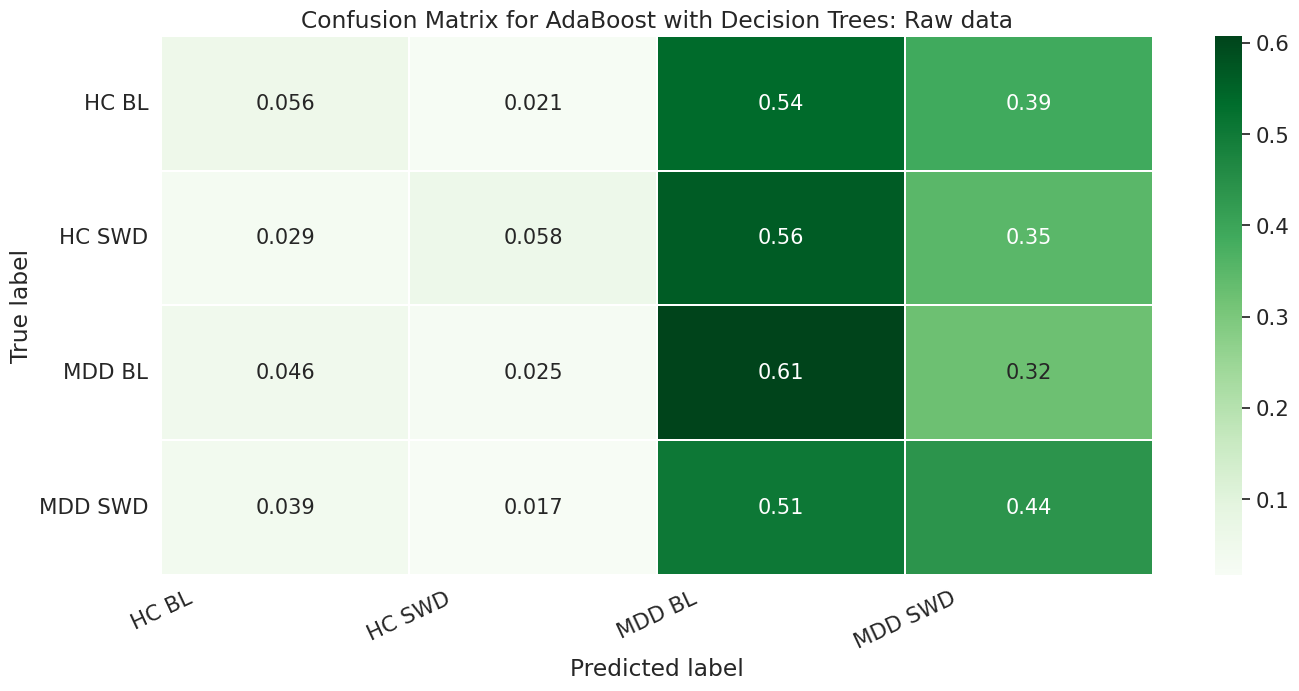
\includegraphics[scale=0.4]{cm-raw}


\justifying
\begin{multicols}{2}

However, it is important to note that the proxy for neuroplasticity in the
double pulse paradigm is precisely the relative amplitude of double pulses with
respect to test pulses. The raw data lacks any measure of relative amplitude.
Besides, regardless of the fact that the model above suggests a critical
difference in the response patterns between subject groups, its accuracy is
still poor.

\subsection{Engineered data}

With the inclusion of the $\rho$ feature, accuracy increases by a factor of
$\approx 2.1$ to $72.6\%$. The inclusion of the $\delta$ feature alone increased
it, in comparison to the raw data, had a more or less equivalent impact,
increasing accuracy to $73.4\%$.


\end{multicols}
\raggedright

~

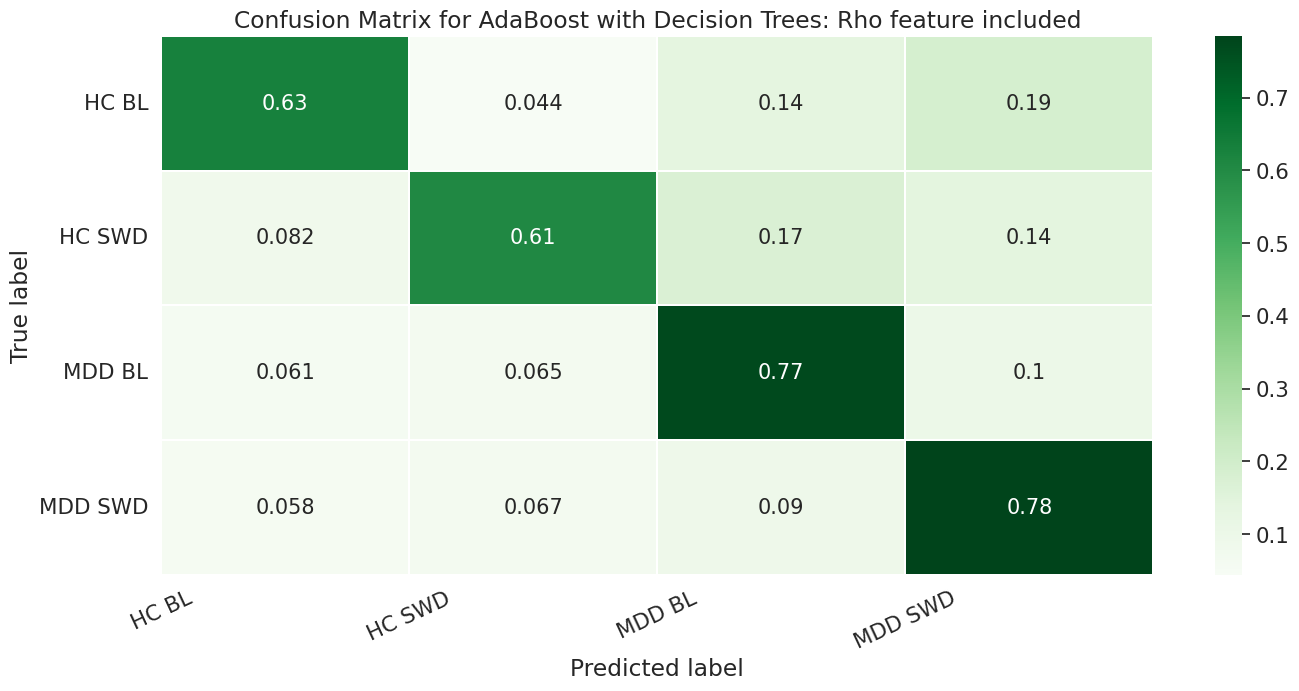
\includegraphics[scale=0.24]{cm-rho}
\raggedright
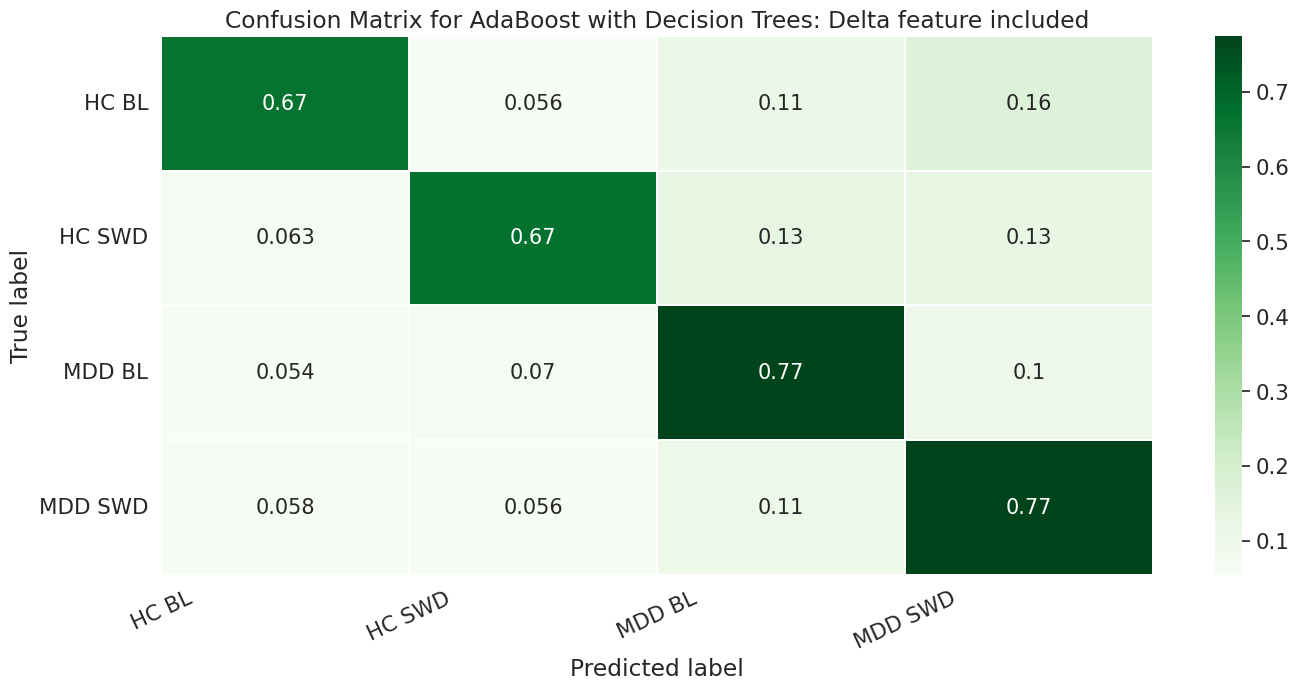
\includegraphics[scale=0.24]{cm-delta}



\justifying
\begin{multicols}{2}

The model still shows a higher accuracy when classifying diagnosed subjects, but
the overall accuracy across all categories was significantly improved.

As stated earlier, the inclusion of the $\delta$ and $\rho$ features computed
over the logarithmically transformed EMG peak-to-peak improved the model's
accuracy. Concretely, accuracy was increased to $86\%$, with the following
confusion matrix.

\end{multicols}

~
\centering

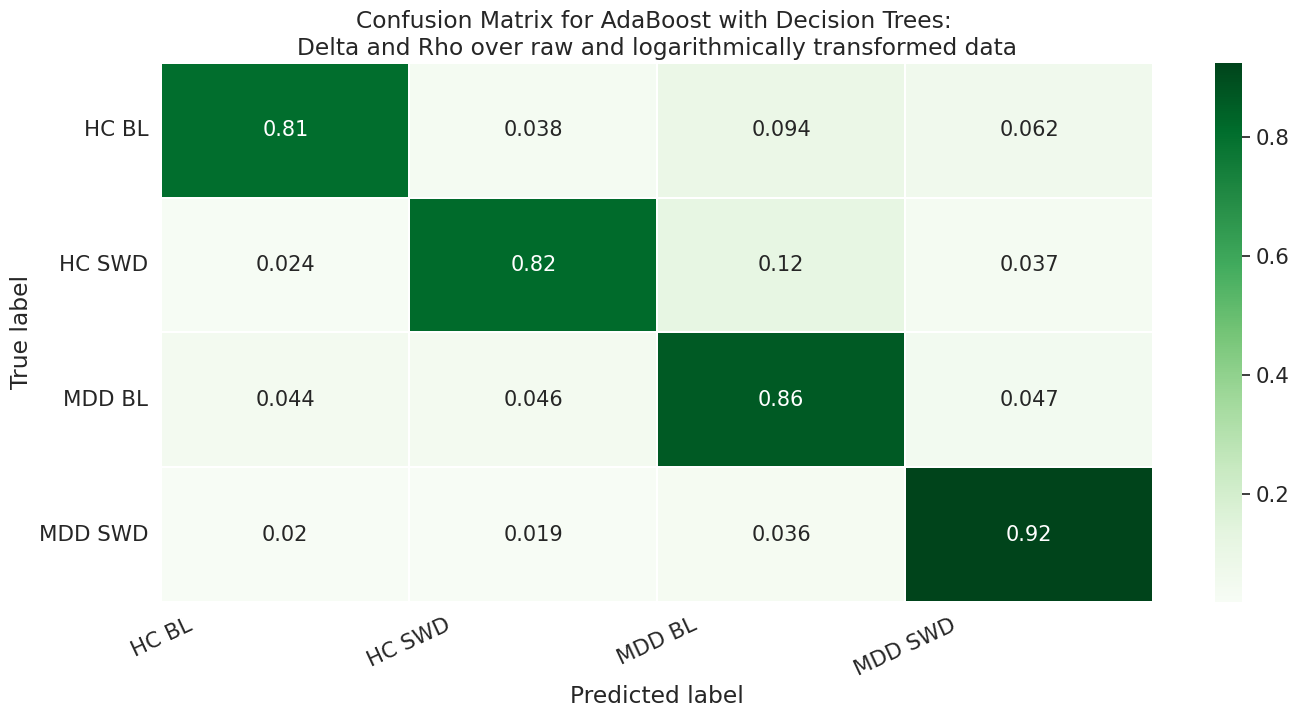
\includegraphics[scale=0.4]{cm-dr-ln}


\justifying
\begin{multicols}{2}

At last, if to the previous model we add also the weighted versions of $\delta$
and $\rho$, using inverse-variance weights, we obtained an accuracy of $89.8\%$,
with the following confusion matrix.

\end{multicols}

\centering
~

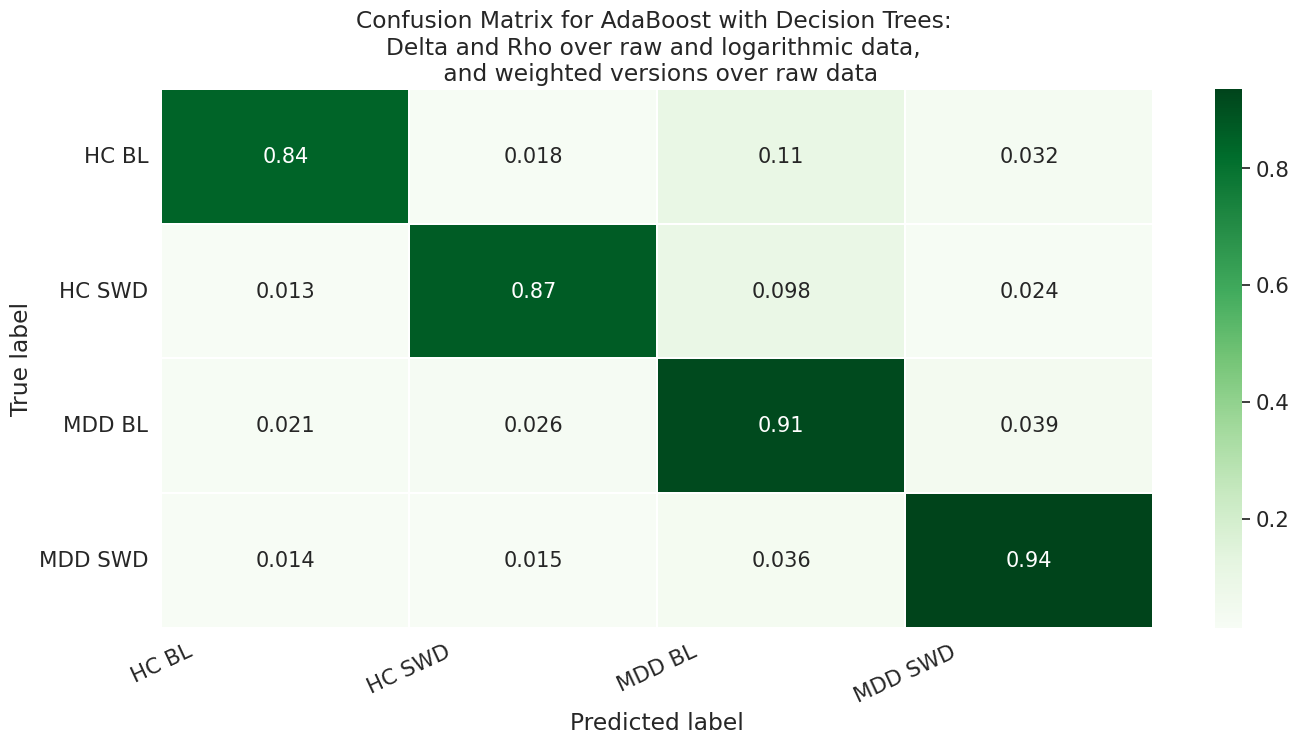
\includegraphics[scale=0.4]{final-cm}


\justifying
\begin{multicols}{2}



\section{Statistics}

\begin{wrnote}
    The description of the experimental process in this section is poor. Also I
    do not know the total number of subjects, experiments are still being
    conducted. Need input from the lab on these matters.
\end{wrnote}


Although distributions were always exponential, the $\beta$ parameter of said
distributions varied across subject groups and session types. 

~

    \begin{tabular}{ |p{2cm}|p{2cm}|p{2cm}|  }
    \hline
    &       Mean & Median \\
    \hline
    HC BL & 196.77 & 149.36 \\
    \hline
    HC SWD & 165.98 & 99.76 \\
    \hline \\ 
    MDD BL & 187.56 & 127.69\\ 
    \hline 
    MDD SWD & 247.57 & 151.07 \\
    \hline
    \end{tabular}

~ 

Each of the means in the above table correspond to the estimated $\beta$
parameter of the distribution of the paired pulses on each subject group.

\end{multicols}
\raggedright

~

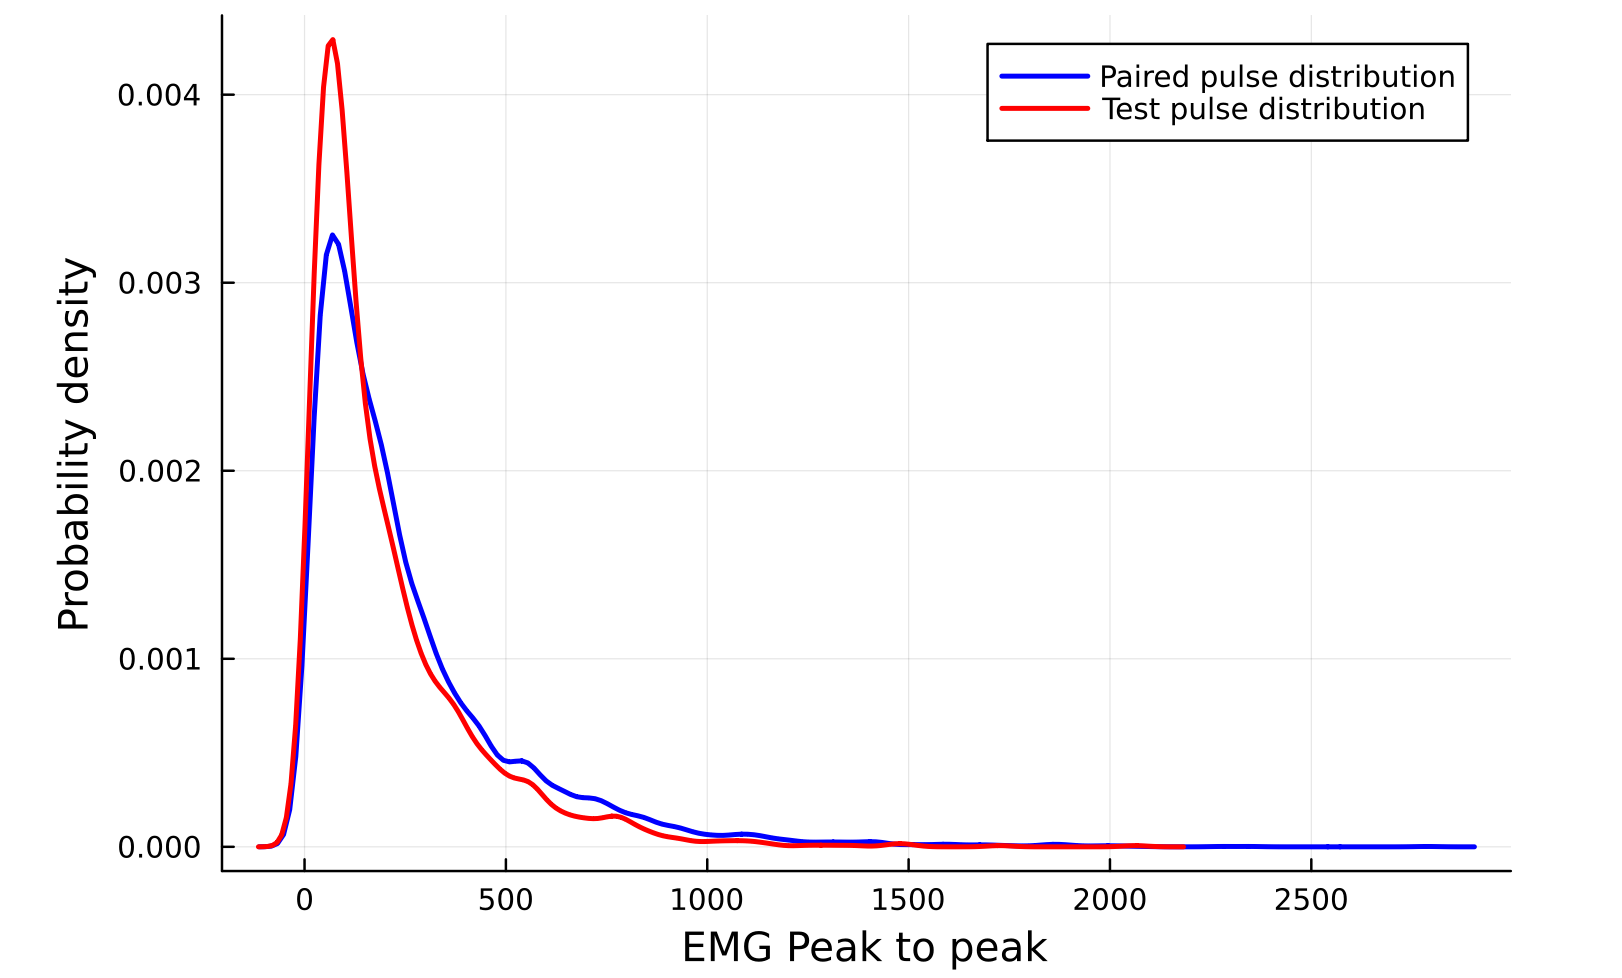
\includegraphics[scale=0.14]{Paired-TestDist}
\raggedright
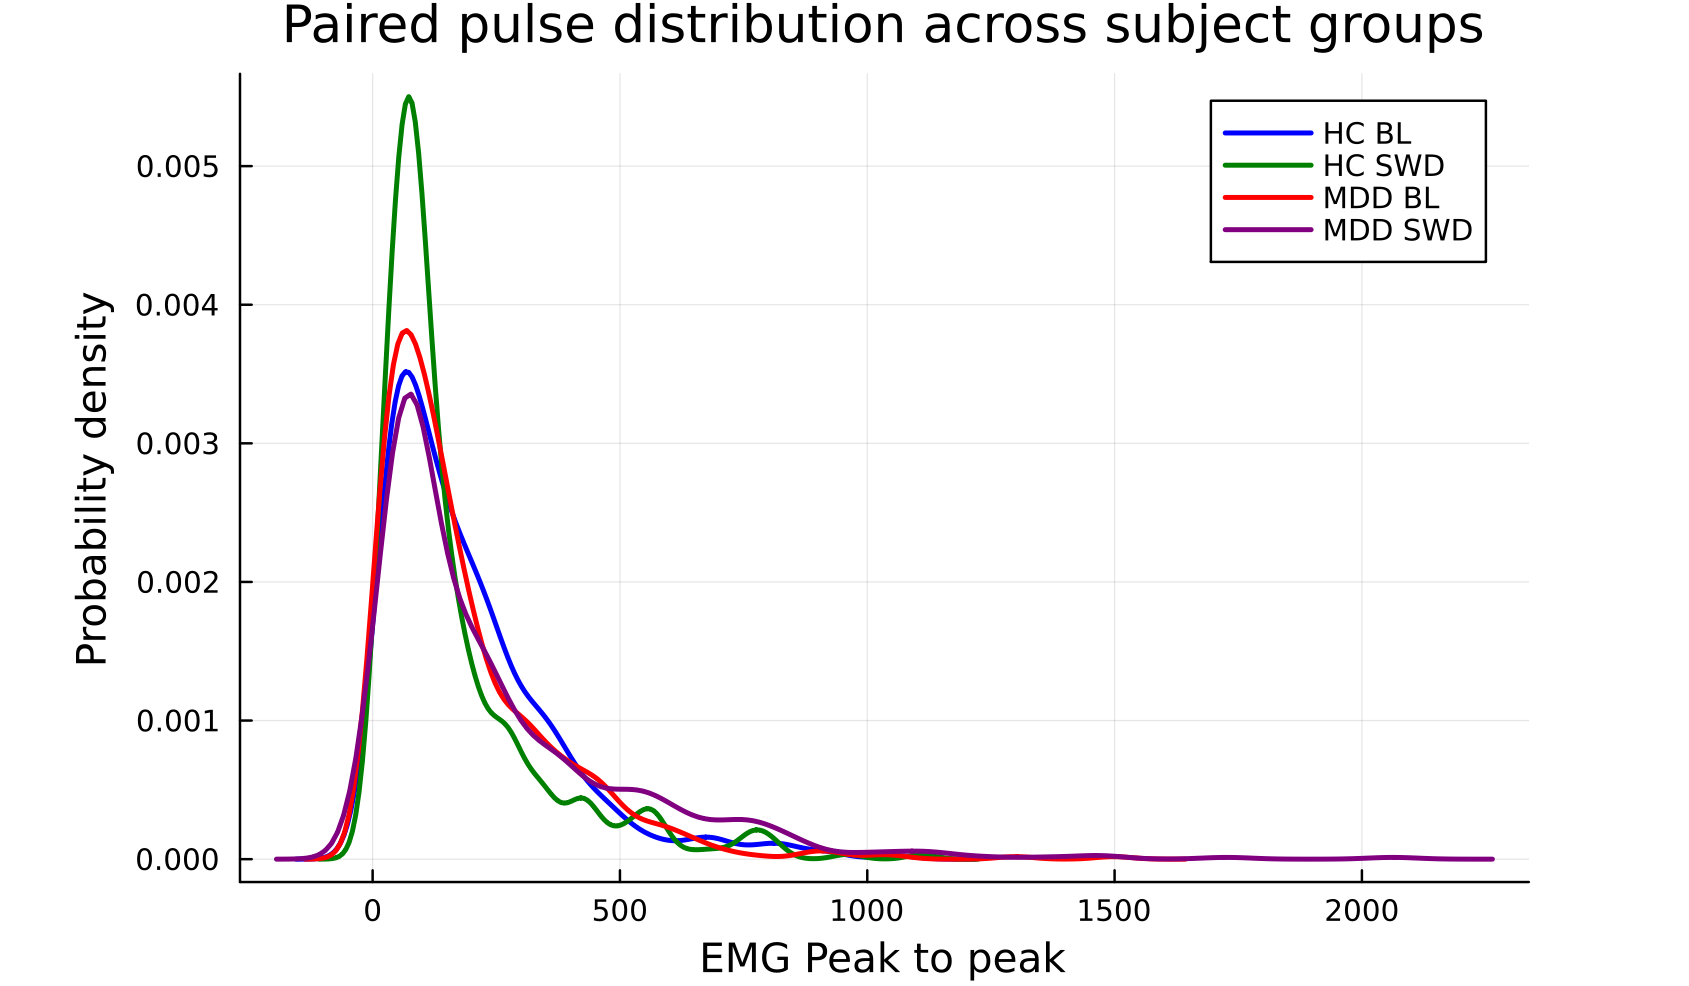
\includegraphics[scale=0.14]{P-dist-subjects-big}



\justifying
\begin{multicols}{2}



\section{Discussion}

The previous results show that the inclusion of pulse-specific relative
amplitude measures greatly improve the accuracy of a random forests model
trained over TMS data for subject classification. More importantly, it becomes
clear that, via the engineered features $\delta$ and $\rho$, researchers can
attain evidence in favour or against hypotheses pertaining to differences among
subject groups. Particularly, in showing that pulse-specific measures of
relative amplitude are significant information to determine the sleep session
and group of a subject, and being relative amplitude measures a proxy for
neuroplasticity, the previous model provides evidence in favour of
sleep-modulated, depression-induced differences in neuroplasticity.

The use of machine learning models over neuroscientific observations is not only
a promising tool in the production of evidence. There is a diagnostic potential
that is still to be evaluated. Indeed, if machine learning models can detect the
neural patterns that distinguish, under specific experimental conditions,
healthy control from diagnosed subjects, such models can potentially be
implemented in the diagnosis process as powerful clinical tool. 

Although long and serious scientific effort is still required to appraise the
diagnostic potential of machine learning models, we believe our results allow
for a certain amount of conservative optimism on the matter.

In short, pulse-specific relative amplitude features are successful in making
machine learning models applicable to TMS experimental data. Thus, they can play
an important part in future research by allowing for new ways of analyzing and
extracting meaningful information of TMS results.

\section{Appendix 1}



\section{Appendix 2}

\textbf{Proof 1}. In \textbf{Remark 1}, we observed the following property:

    \begin{align*}
        \forall x: x \in \mathbb{R}^+ : \delta(x) \geq \rho(x)
    .\end{align*}

Such property can be proven via induction. Firstly, recall that


\begin{align*} \delta(x) &= \frac{x}{m}\sum^m\frac{1}{t_j} \\
                \rho(x) &= \frac{xm}{\sum^m t_j} \end{align*}


Let $S_1^m = \sum^m\frac{1}{t_j}, S_2^m= \sum^m t_j$. We operate under the
assumption that $t_i \in \mathbb{R}^+$. It is the case that

\begin{align*} 
    \frac{x}{m}\sum^m\frac{1}{t_j} &\geq \frac{xm}{\sum^m t_j} \\ 
    S_2^mS_1^m &\geq m^2
\end{align*}

This holds for $m=1$, since $\frac{1}{t_1}+t_1 \geq 1 \iff 1+t_1^2 \geq t_1$. So
we may assume $S^k_1 S^k_2 \geq k^2$ . We now set out to show that

\begin{equation*} 
    S^{k+1}_1 S^{k+1}_2 \geq (k+1)^2
\end{equation*}

This can be proven as follows.

\begin{align*} 
    S^{k+1}_1 S^{k+1}_2 &\geq (k+1)^2 \\ 
    (S_1^k+\frac{1}{t_{t+1}})(S_2^k+t_{k+1}) &\geq k^2+2k+1 \\
    S^k_1S^k_2+ t_{k+1}S_1^k + \frac{1}{t_{k+1}}S^k_2+1 &\geq k^2+2k+1 \\
    S^k_1S^k_2+ t_{k+1}S_1^k + \frac{1}{t_{k+1}}S^k_2 &\geq k^2+2k 
\end{align*}

We know $S^k_1S^k_2 \geq k^2$ and then it suffices to show $t_{k+1}S_1^k +
\frac{S^k_2}{t_{k+1}}\geq 2k$. To prove this, simply observe that

\begin{align*}
    \frac{1}{t_{k+1}}\sum_{j=1}^mt_j+t_{k+1}\sum_{j=1}^m\frac{1}{t_{j}} &\geq 2k \\
    \Big(\frac{t_1}{t_{k+1}}+...+\frac{t_k}{t_{k+1}}\Big)+\Big(\frac{t_{k+1}}{t_1}+...+\frac{t_{k+1}}{t_k}\Big)
    &\geq 2k \\ \iff
    \overbrace{a+\frac{1}{a}+b+\frac{1}{b}+... +
    n+\frac{1}{n}}^{\text{$2k$ terms} } &\geq 2k
\end{align*}

We have $\min f=2$  for $f(x)=x+\frac{1}{x}$ for $x \in \mathbb{R}^+$. Then
$\min(a+\frac{1}{a}+...+n+\frac{1}{n})=2k$ for $a,..., n \in \mathbb{R}^+$,
which concludes the demonstration.

\end{document}

